% Template for USENIX papers.
%
% History:
%
% - TEMPLATE for Usenix papers, specifically to meet requirements of
%   USENIX '05. originally a template for producing IEEE-format
%   articles using LaTeX. written by Matthew Ward, CS Department,
%   Worcester Polytechnic Institute. adapted by David Beazley for his
%   excellent SWIG paper in Proceedings, Tcl 96. turned into a
%   smartass generic template by De Clarke, with thanks to both the
%   above pioneers. Use at your own risk. Complaints to /dev/null.
%   Make it two column with no page numbering, default is 10 point.
%
% - Munged by Fred Douglis <douglis@research.att.com> 10/97 to
%   separate the .sty file from the LaTeX source template, so that
%   people can more easily include the .sty file into an existing
%   document. Also changed to more closely follow the style guidelines
%   as represented by the Word sample file.
%
% - Note that since 2010, USENIX does not require endnotes. If you
%   want foot of page notes, don't include the endnotes package in the
%   usepackage command, below.
% - This version uses the latex2e styles, not the very ancient 2.09
%   stuff.
%
% - Updated July 2018: Text block size changed from 6.5" to 7"
%
% - Updated Dec 2018 for ATC'19:
%
%   * Revised text to pass HotCRP's auto-formatting check, with
%     hotcrp.settings.submission_form.body_font_size=10pt, and
%     hotcrp.settings.submission_form.line_height=12pt
%
%   * Switched from \endnote-s to \footnote-s to match Usenix's policy.
%
%   * \section* => \begin{abstract} ... \end{abstract}
%
%   * Make template self-contained in terms of bibtex entires, to allow
%     this file to be compiled. (And changing refs style to 'plain'.)
%
%   * Make template self-contained in terms of figures, to
%     allow this file to be compiled. 
%
%   * Added packages for hyperref, embedding fonts, and improving
%     appearance.
%   
%   * Removed outdated text.
%
%%%%%%%%%%%%%%%%%%%%%%%%%%%%%%%%%%%%%%%%%%%%%%%%%%%%%%%%%%%%%%%%%%%%%%%%%%%%%%%%

\documentclass[letterpaper,twocolumn,10pt]{article}
\usepackage{../usenix2019_v3}

% to be able to draw some self-contained figs
\usepackage{tikz}
\usepackage{amsmath}
\usepackage{url}

% Figures live in ../figures/ (project-level report/figures/). graphicspath
% lets us reference them by bare filename — \includegraphics{04_viz__...}
% rather than \includegraphics{../figures/04_viz__...}.
\usepackage{graphicx}
\graphicspath{{../figures/}}

% inlined bib file
\usepackage{filecontents}

%-------------------------------------------------------------------------------
\begin{filecontents}{\jobname.bib}
%-------------------------------------------------------------------------------
@Article{yang2019arming,
  author =       {Yang, Kai-Cheng and Varol, Onur and Davis, Clayton A. and Ferrara, Emilio and Flammini, Alessandro and Menczer, Filippo},
  title =        {Arming the Public with Artificial Intelligence to Counter Social Bots},
  journal =      {Human Behavior and Emerging Technologies},
  year =         2019,
  volume =       {1},
  number =       {1},
  pages =        {48--61},
  note =         {\url{https://doi.org/10.1002/hbe2.115}}
}

@Article{ferrara2016rise,
  author =       {Ferrara, Emilio and Varol, Onur and Davis, Clayton and Menczer, Filippo and Flammini, Alessandro},
  title =        {The Rise of Social Bots},
  journal =      {Communications of the ACM},
  year =         2016,
  volume =       {59},
  number =       {7},
  pages =        {96--104},
  note =         {\url{https://doi.org/10.1145/2818717}}
}

@Article{cresci2020decade,
  author =       {Cresci, Stefano},
  title =        {A Decade of Social Bot Detection},
  journal =      {Communications of the ACM},
  year =         2020,
  volume =       {63},
  number =       {10},
  pages =        {72--83},
  note =         {\url{https://doi.org/10.1145/3409116}}
}

@InProceedings{cresci2017paradigm,
  author =       {Cresci, Stefano and Di Pietro, Roberto and Petrocchi, Marinella and Spognardi, Angelo and Tesconi, Maurizio},
  title =        {The Paradigm-Shift of Social Spambots: Evidence, Theories, and Tools for the Arms Race},
  booktitle =    {Proceedings of the 26th International Conference on World Wide Web Companion (WWW '17 Companion)},
  year =         2017,
  pages =        {963--972},
  note =         {\url{https://doi.org/10.1145/3041021.3055135}}
}

@InProceedings{feng2021twibot20,
  author =       {Feng, Shangbin and Wan, Herun and Wang, Ningnan and Li, Jundong and Luo, Minnan},
  title =        {{TwiBot-20}: A Comprehensive {Twitter} Bot Detection Benchmark},
  booktitle =    {Proceedings of the 30th ACM International Conference on Information and Knowledge Management (CIKM '21)},
  year =         2021,
  pages =        {4485--4494},
  note =         {\url{https://doi.org/10.1145/3459637.3482019}}
}

@InProceedings{feng2022twibot22,
  author =       {Feng, Shangbin and Tan, Zhaoxuan and Wan, Herun and Wang, Ningnan and Chen, Zilong and Zhang, Binchi and Zheng, Qinghua and Zhang, Wenqian and Lei, Zhenyu and Yang, Shujie and Feng, Xinshun and Zhang, Qingyue and Wang, Hongrui and Liu, Yuhan and Bai, Yuyang and Wang, Heng and Cai, Zijian and Wang, Yanbo and Zheng, Lijing and Ma, Zihan and Li, Jundong and Luo, Minnan},
  title =        {{TwiBot-22}: Towards Graph-Based {Twitter} Bot Detection},
  booktitle =    {Proceedings of the 36th Conference on Neural Information Processing Systems (NeurIPS 2022) Datasets and Benchmarks Track},
  year =         2022,
  note =         {\url{https://twibot22.github.io/}}
}

@Article{shao2018spread,
  author =       {Shao, Chengcheng and Ciampaglia, Giovanni Luca and Varol, Onur and Yang, Kai-Cheng and Flammini, Alessandro and Menczer, Filippo},
  title =        {The Spread of Low-Credibility Content by Social Bots},
  journal =      {Nature Communications},
  year =         2018,
  volume =       {9},
  pages =        {4787},
  note =         {\url{https://doi.org/10.1038/s41467-018-06930-7}}
}

@Article{yang2022botometer,
  author =       {Yang, Kai-Cheng and Ferrara, Emilio and Menczer, Filippo},
  title =        {Botometer 101: Social Bot Practicum for Computational Social Scientists},
  journal =      {Journal of Computational Social Science},
  year =         2022,
  volume =       {5},
  number =       {2},
  pages =        {1511--1528},
  note =         {\url{https://doi.org/10.1007/s42001-022-00177-5}}
}

@Article{bessi2016distort,
  author =       {Bessi, Alessandro and Ferrara, Emilio},
  title =        {Social Bots Distort the 2016 {U.S.} Presidential Election Online Discussion},
  journal =      {First Monday},
  year =         2016,
  volume =       {21},
  number =       {11},
  note =         {\url{https://doi.org/10.5210/fm.v21i11.7090}}
}

@Article{ferrara2017french,
  author =       {Ferrara, Emilio},
  title =        {Disinformation and Social Bot Operations in the Run Up to the 2017 {French} Presidential Election},
  journal =      {First Monday},
  year =         2017,
  volume =       {22},
  number =       {8},
  note =         {\url{https://doi.org/10.5210/fm.v22i8.8005}}
}

@Article{alazawi2022feature,
  author =       {Al-Azawi, Raad Ghazi and AL-mamory, Safaa O.},
  title =        {Feature Extractions and Selection of Bot Detection on {Twitter}: A Systematic Literature Review},
  journal =      {Inteligencia Artificial},
  year =         2022,
  volume =       {25},
  number =       {69},
  pages =        {57--86},
  note =         {\url{https://doi.org/10.4114/intartif.vol25iss69pp57-86}}
}

\end{filecontents}

%-------------------------------------------------------------------------------
\begin{document}
%-------------------------------------------------------------------------------

%don't want date printed
\date{}

% make title bold and 14 pt font (Latex default is non-bold, 16 pt)
\title{\Large \bf Detecting Social Media Bots via Reinforcement Learning}

%for single author (just remove % characters)
\author{
{\rm Ahtesham Alvi}\\
aalvi1@terpmail.umd.edu
\and
{\rm Declan Scott}\\
djscott@terpmail.umd.edu
\\
\and
{\rm Michael Morton}\\
mmorton4@terpmail.
umd.edu
\and
{\rm Tristan Tang}\\
ttsang@terpmail.umd.edu
\\
\and
{\rm Yudhiishbala Senthilkumar}\\
yudhiish@terpmail.umd.edu
\\
}
% copy the following lines to add more authors
% \and
% {\rm Name}\\
%Name Institution
% end author

\maketitle

%-------------------------------------------------------------------------------
\begin{abstract}
%-------------------------------------------------------------------------------
% TODO: 150-250 words. State the problem (cross-era bot detection),
% the gap (no published study trains on one era and evaluates on the
% next), the approach (canonical feature pipeline + pairwise model
% schema + cross-era evaluation matrix), and the headline finding.
\textit{Abstract goes here.}
\end{abstract}

%-------------------------------------------------------------------------------
\section{Introduction}\label{sec:intro}
%-------------------------------------------------------------------------------
% TODO: motivation, problem statement, and a short roadmap of the paper.
% Should end with an explicit list of contributions.
\textit{Introduction goes here.}

\paragraph{Contributions.}
% TODO: replace with real bullet list once the experiments settle.
\begin{itemize}
  \item \textit{Contribution 1.}
  \item \textit{Contribution 2.}
  \item \textit{Contribution 3.}
\end{itemize}

%-------------------------------------------------------------------------------
\section{Related Work}\label{sec:related}
%-------------------------------------------------------------------------------
% TODO: organize by theme — (a) bot detection surveys, (b) benchmark
% datasets, (c) feature- and graph-based detection methods, (d) studies
% of real-world bot impact. The grouped \cite calls below are stubs that
% keep the bibliography populated until the prose is written; replace
% them with proper in-text references.
Foundational surveys frame the bot-detection
problem~\cite{ferrara2016rise,cresci2020decade,alazawi2022feature}.
Benchmark datasets define the empirical
landscape~\cite{cresci2017paradigm,feng2021twibot20,feng2022twibot22}.
Behavioural-feature and tool-based detection
methods~\cite{yang2019arming,yang2022botometer} establish the
single-dataset baseline this work builds on. Studies of real-world bot
activity in political events motivate the cross-era
question~\cite{bessi2016distort,ferrara2017french,shao2018spread}.

%-------------------------------------------------------------------------------
\section{Datasets}\label{sec:datasets}
%-------------------------------------------------------------------------------
% TODO: per-dataset table (rows = datasets, cols = users, tweets, bot rate,
% collection year). Discuss feature availability differences (twibot_2020
% has no in_reply_to_user_id, cresci_2017 has no follow graph, etc.) and
% how the canonical schema handles them.
\textit{Dataset descriptions go here.}

%-------------------------------------------------------------------------------
\section{Feature Engineering}\label{sec:fe}
%-------------------------------------------------------------------------------
% TODO: account features, tweet behavioural features, graph features,
% per-day rates, NaN-vs-0 semantics, the cross-era feature contract.
\textit{Feature engineering pipeline goes here.}

%-------------------------------------------------------------------------------
\section{Methodology}\label{sec:method}
%-------------------------------------------------------------------------------
% TODO: pairwise (train, test) experimental setup, the six classifier
% families, train/test split convention (full set off-diagonal,
% stratified 80/20 on the diagonal), the per-pair feature schema.
\textit{Methodology goes here.}

%-------------------------------------------------------------------------------
\section{Experiments and Results}\label{sec:results}
%-------------------------------------------------------------------------------
% TODO: AUC matrices per model, the bots-over-time headline plot,
% feature importance shifts. Reference figures by \ref{...} so the
% numbering stays consistent if figures are reordered.
\textit{Results discussion goes here.}

% --- Example: linking a figure from report/figures/ -----------------------
% Because the preamble sets \graphicspath{{../figures/}}, we reference the
% figure by bare filename (no path, no extension required if the file is
% PNG/PDF/JPG). Cross-reference via \ref{fig:bots-over-time}.
\begin{figure}[t]
  \centering
  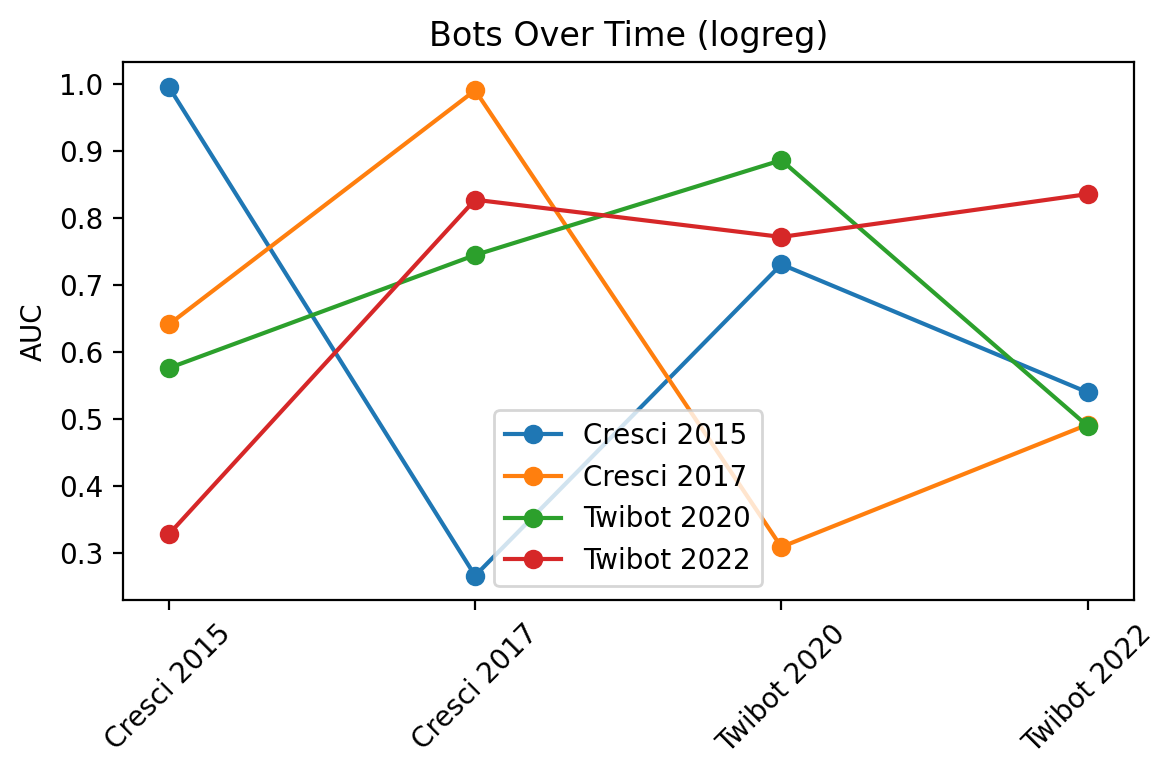
\includegraphics[width=\columnwidth]{04_viz__story__bots_over_time_logreg}
  \caption{%
    Cross-era AUC for a logistic-regression bot detector. Each line is
    one training dataset; the x-axis is the test dataset in chronological
    order. \textit{TODO: rewrite caption with real numbers once results
    are final.}%
  }
  \label{fig:bots-over-time}
\end{figure}
% Use \ref{fig:bots-over-time} in body prose (e.g. ``see
% Figure~\ref{fig:bots-over-time}''). For a full-page-width figure that
% spans both columns, use \begin{figure*}...\end{figure*} instead.

%-------------------------------------------------------------------------------
\section{Discussion}\label{sec:discussion}
%-------------------------------------------------------------------------------
% TODO: what do the cross-era trends actually mean for bot evolution?
% Where does the model fail (which (train, test) pairs degrade most)?
% What do the feature-importance shifts say about how bots changed?
\textit{Discussion goes here.}

%-------------------------------------------------------------------------------
\section{Limitations}\label{sec:limitations}
%-------------------------------------------------------------------------------
% TODO: dataset-comparability caveats (label semantics across cresci/
% twibot, scale shift in raw counts, graph-construction differences),
% the modern-data-collection gap (post-2022 X API restrictions).
\textit{Limitations go here.}

%-------------------------------------------------------------------------------
\section{Conclusion}\label{sec:conclusion}
%-------------------------------------------------------------------------------
% TODO: 1-paragraph summary + future work pointer.
\textit{Conclusion goes here.}

%-------------------------------------------------------------------------------
\bibliographystyle{plain}
\bibliography{\jobname}

%%%%%%%%%%%%%%%%%%%%%%%%%%%%%%%%%%%%%%%%%%%%%%%%%%%%%%%%%%%%%%%%%%%%%%%%%%%%%%%%
\end{document}
%%%%%%%%%%%%%%%%%%%%%%%%%%%%%%%%%%%%%%%%%%%%%%%%%%%%%%%%%%%%%%%%%%%%%%%%%%%%%%%%

%%  LocalWords:  endnotes includegraphics fread ptr nobj noindent
%%  LocalWords:  pdflatex acks